\documentclass[xcolor=x11names,compress,usenames,dvipsnames,mathsans]{beamer}
\usepackage[utf8]{inputenc}
\usepackage{stmaryrd}
\usepackage{tikz}
\usepackage{listings}
\usepackage{textpos}
\usepackage[english]{babel}
\usepackage{natbib}
\usepackage{wrapfig,color,dashrule,epsfig,graphicx}
\usepackage{pstool,psfrag}
\newcommand{\calt}{\color{red} } % alert color
\newcommand{\ccom}{\color{blue} } % commentary color

\newcommand{\redtext}[1]{\color{UOEred}{#1}\color{UOEblue}}

\newcommand{\link}[1]{\textbf{\textcolor{PMS3025}{\underline{#1}}}}
\definecolor{NewRed}{rgb}{0.8, 0.0, 0.0}


 %% Beamer Layout %%%%%%%%%%%%%%%%%%%%%%%%%%%%%%%%%%
\usetheme{Edinburgh}
\usecolortheme{edinburgh}
\usefonttheme[onlylarge]{structurebold}
\setbeamertemplate{itemize items}[circle]

\setbeamerfont{title}{size={\fontsize{13}{20}}}
\setbeamercolor*{palette tertiary}{fg=black,bg=black!10}
\setbeamercolor*{palette quaternary}{fg=black,bg=black!10}
\setbeamercolor{alerted text}{fg=red}
\setbeamercolor{sidebar}{bg=red!25!blue,fg=white}

\def\ci{\perp\!\!\!\perp}

\setbeamercovered{transparent}

\addtobeamertemplate{footline}{}
{
  \begin{textblock*}{100mm}(.845\textwidth,-0.57cm)
    \includegraphics[height=0.5cm, width=1.8cm]{225px-Epcc_logo.jpg}
  \end{textblock*}
}



\addtobeamertemplate{frametitle}{}
{
  \begin{textblock*}{100mm}(.935\textwidth,-0.645cm)
	\includegraphics[scale=.1]{crest_rb.eps}
  \end{textblock*}
}


\usepackage{graphicx} % Allows including images
\usepackage{booktabs} % Allows the use of \toprule, \midrule and \bottomrule in tables



%\setbeamercovered{transparent}

%----------------------------------------------------------------------------------------
%	STYLE STUFF -- section title slides
%----------------------------------------------------------------------------------------

\AtBeginSection[]{
  \begin{frame}
  \vfill
  \centering
  \begin{beamercolorbox}[sep=8pt,center,shadow=true,rounded=true]{title}
    \usebeamerfont{title}\insertsectionhead\par%
  \end{beamercolorbox}
  \vfill
  \end{frame}
}

\bibliographystyle{abbrv}


\title{A tensorflow backened to SpiNNaker \\
  More precicely: a keras backend to SpiNNaker}

\author[author]{Jonas Fassbender \\
\textit{jonas@fassbender.dev} \\
\vspace{1em}
\includegraphics[scale=.8]{logo_colour.pdf}
}

\date{}

\begin{document}

% titlepage {{{
\begin{frame}
  \titlepage
  \vspace{-2cm}

  \begin{center}
  Supervisors:

  Alan Stokes, Kevin Stratford, Caoimhín Laoide-Kemp
  \end{center}
\end{frame}
% }}}

% What is SpiNNaker? {{{
\section{SpiNNaker}

\begin{frame}[fragile]
  \frametitle{SpiNNaker}
  \setbeamercovered{invisible}

  \begin{center}
    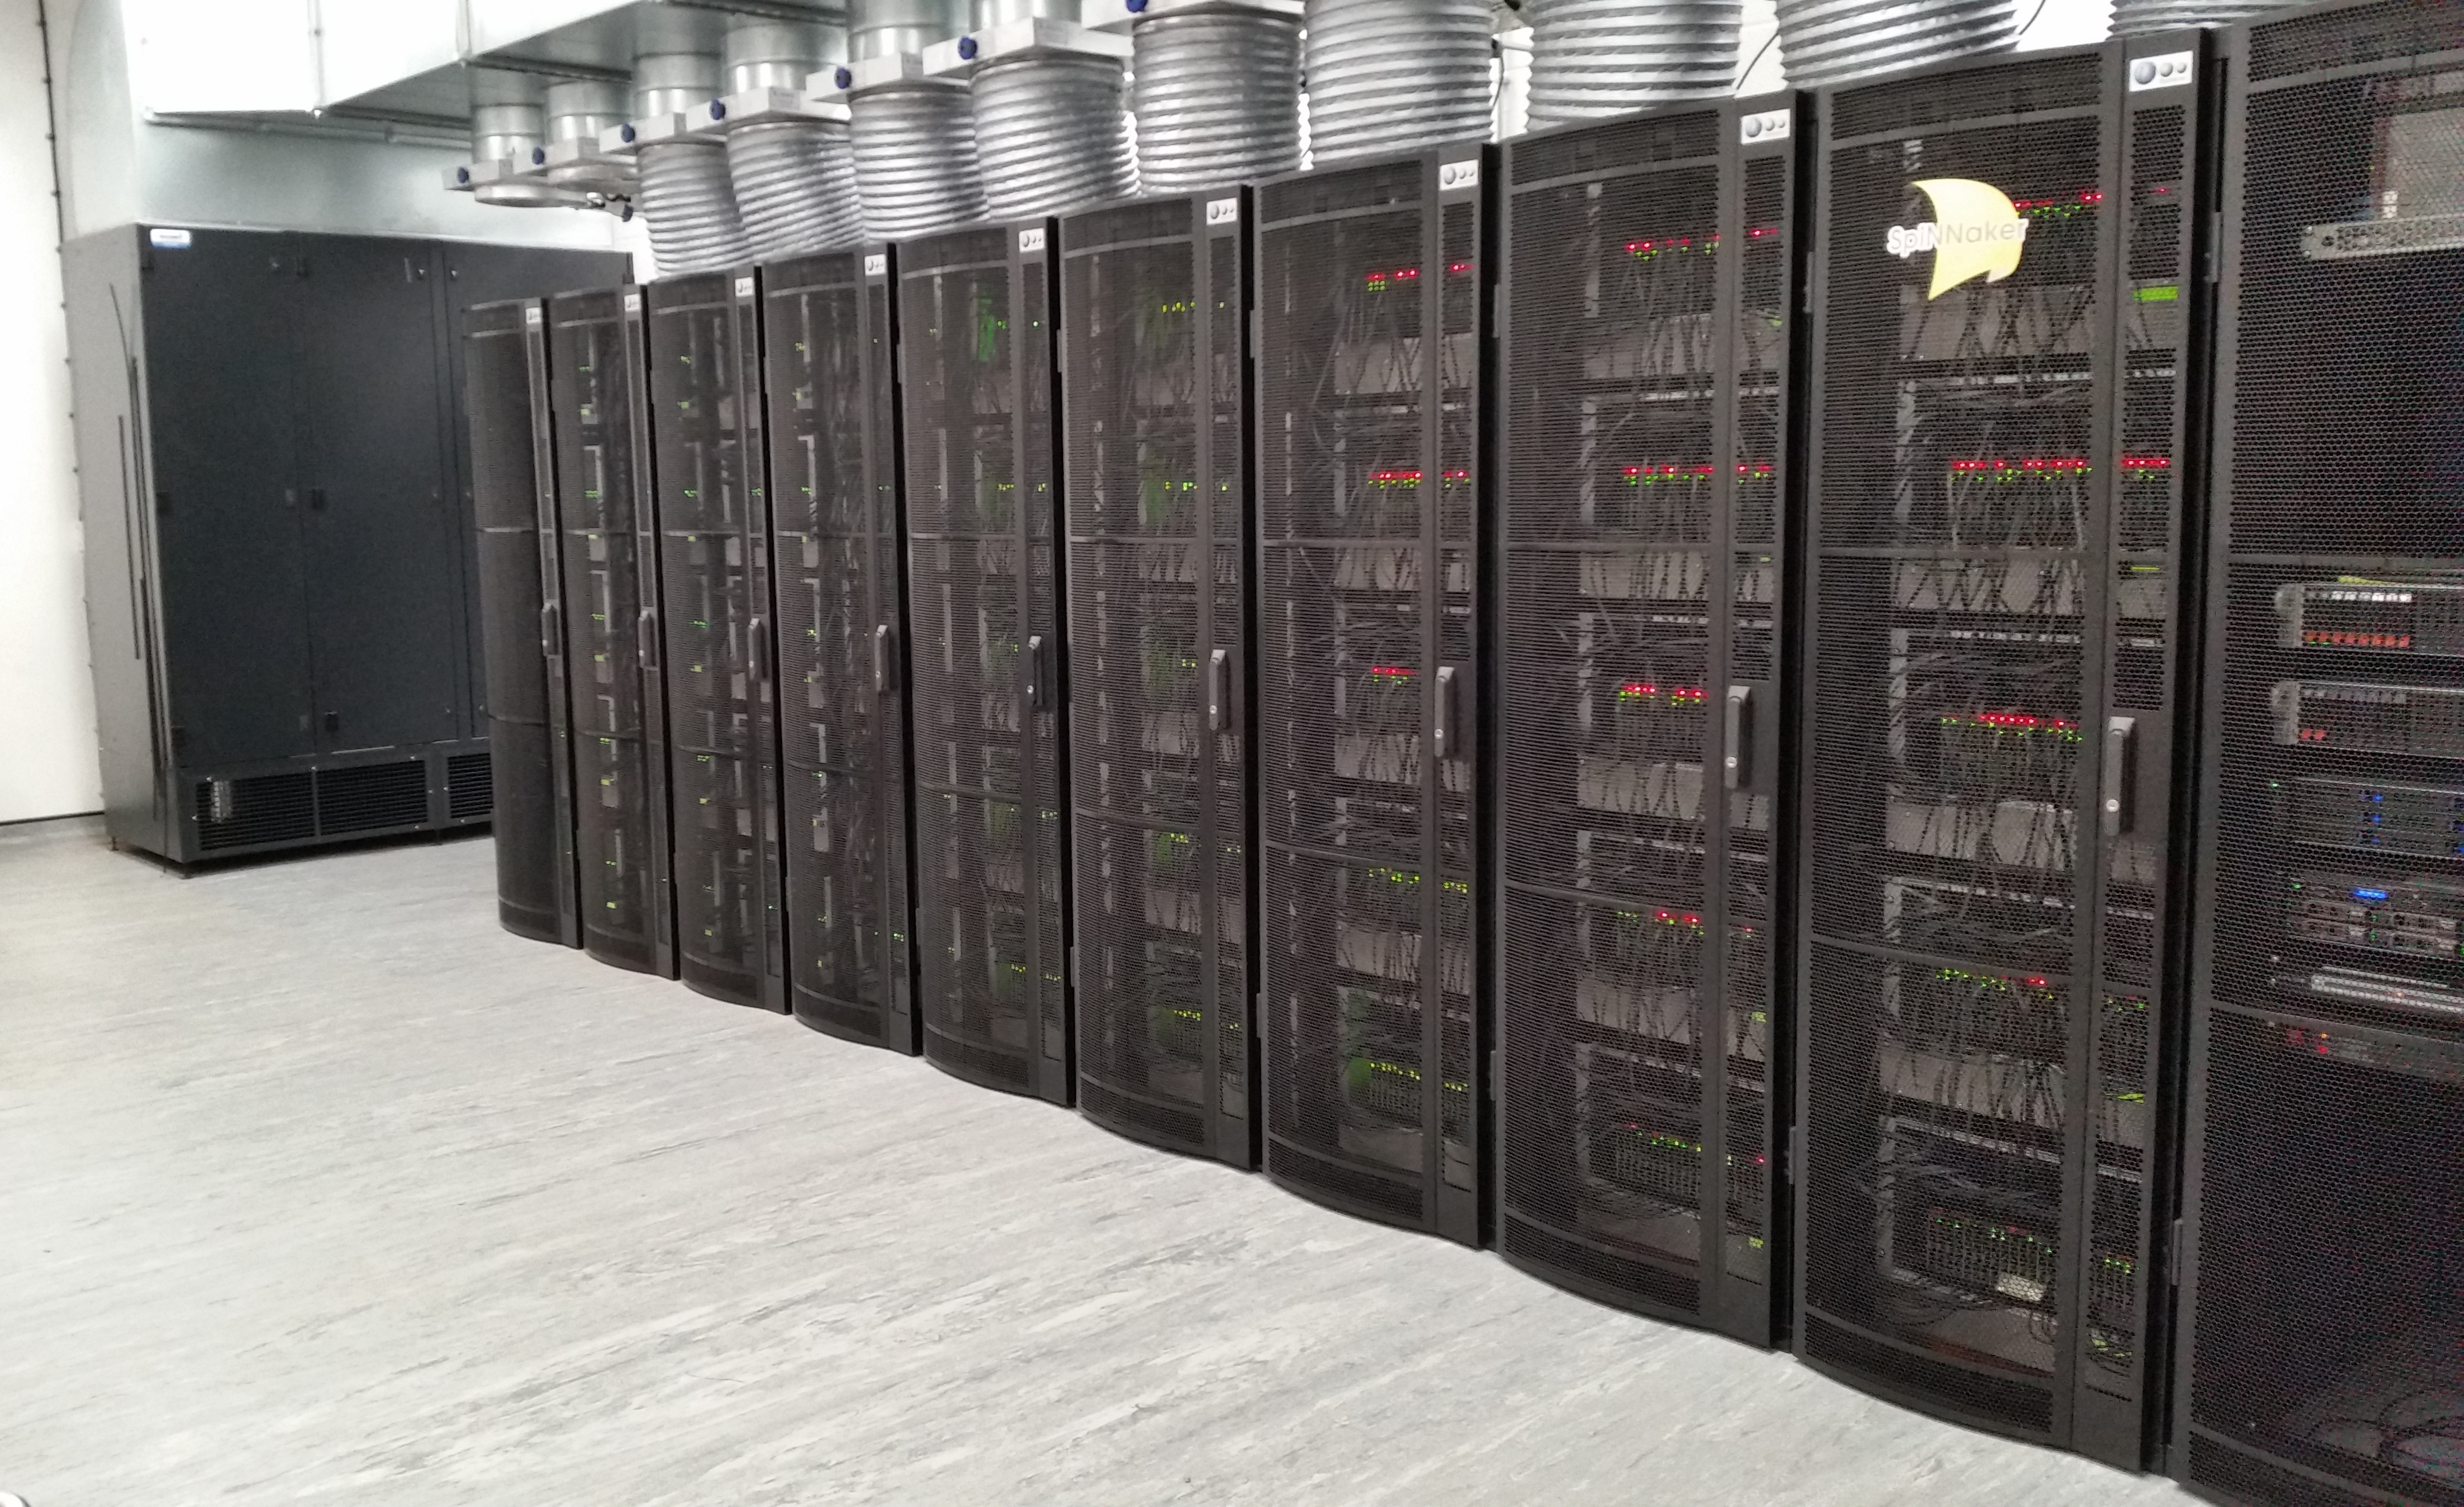
\includegraphics[width=.7\linewidth]
      {SpiNNaker_9cabinets.jpg}
  \end{center}

  [SpiNNaker is] a platform for high-performance massively
  parallel [and energy efficient] processing appropriate
  for the simulation of large-scale [spiking] neural
  networks \cite{spinnaker_project}

\end{frame}
% }}}

% Why use SpiNNaker as a target for training deep NNs? {{{
\section{Motivation}

\begin{frame}[fragile]
  \frametitle{SpiNNaker as a target for training DNNs}
  \setbeamercovered{invisible}

  \begin{itemize}[<+->]
    \item Amount of computation in training DNNs
          increases exponentially (double every 3.4 months)
          \cite{openai2019}
    \item We'll run out of available computation (and
          energy) eventually
    \item Massively parallel, energy efficient and scalable
          systems are optimal for training DNNs
  \end{itemize}
\end{frame}
% }}}

% What is tensorflow? {{{
\section{Tensorflow}

\begin{frame}[fragile]
  \frametitle{Tensorflow}
  \setbeamercovered{invisible}

  \begin{itemize}[<+->]
    \item TensorFlow: Large-Scale Machine Learning on
          Heterogeneous Distributed Systems \cite{tf_2015}
    \item Basically: abstraction over various hardware and
          software libraries and APIs
    \item ``Easiest'' way to add new tensorflow backend? XLA
          (\url{https://www.tensorflow.org/xla})
    \item Instead: backend for keras (\url{https://keras.io})
    \item Using high level conceptual graph (the actual
          layers of the NN) instead of low level
          computational graph of tensorflow
  \end{itemize}
\end{frame}
% }}}

% Challenges {{{
\section{Challenges}

\begin{frame}[fragile]
  \frametitle{Challenges}
  \setbeamercovered{invisible}

  \begin{itemize}[<+->]
    \item Writing scientific programs is hard
    \item Writing programs for embedded hardware is hard
    \item Both together? \dots
  \end{itemize}
\end{frame}
% }}}

% Overcoming them {{{
\section{Overcoming them}

\begin{frame}[fragile]
  \frametitle{Overcoming them}
  \setbeamercovered{invisible}

  \begin{itemize}[<+->]
    \item Prepare myself well
    \item Taking stimulants and don't sleep for three
          months
  \end{itemize}
\end{frame}
% }}}

% References {{{
\begin{frame}
  \frametitle{References}
  \bibliography{literature.bib}
\end{frame}
% }}}

\end{document}
